% Chapter Template

\chapter{Performance Evaluation} % Main chapter title

\label{Chapter5} % Change X to a consecutive number; for referencing this chapter elsewhere, use \ref{ChapterX}
In this section, we explain the setup of our two experiment scenarios and we present the positioning results of our experiments in detail.

%----------------------------------------------------------------------------------------
%	SECTION 1
%----------------------------------------------------------------------------------------

\section{Experiment Setup}
We tested our implementation in two complex indoor scenarios with trajectories through numerous rooms on one floor in a real building of the University of Bern, at Neubrückstrasse 10 in
3012 Bern. The first scenario used an area of $715m^2$ and the second scenario $358m^2$. We distributed the UWB anchor nodes over several rooms to cover the area of interest homogenously.
\begin{figure}[th]
\centering
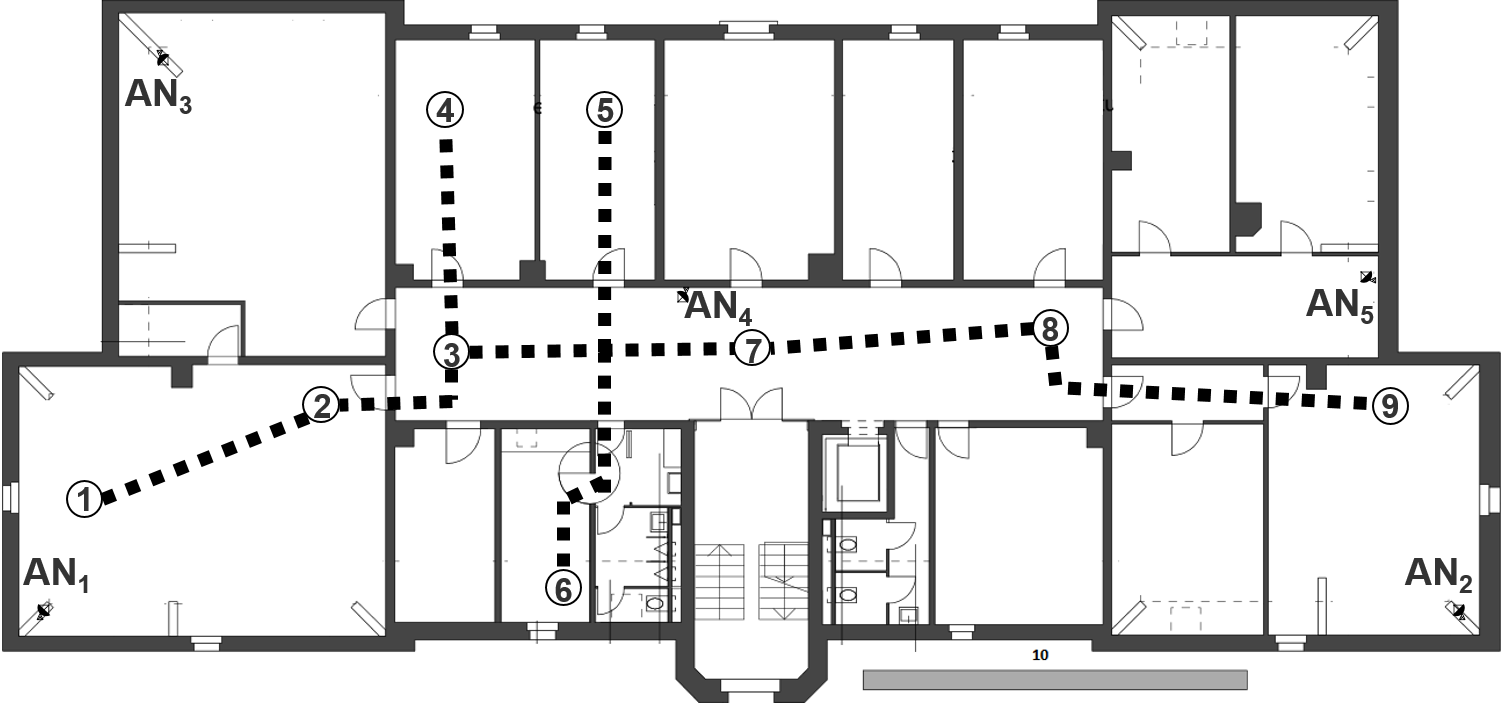
\includegraphics[width=0.8\textwidth]{Figures/trajectory1_withAnchors}
\decoRule
\caption[Anchor Node Positions of Scenario 1]{Trajectory 1 and distributed ANs in scenario 1 on the floor map (with distance reference of 10m).}
\label{fig:trajectory1_withAnchors}
\end{figure}The exact position is indicated in the floor plan of Figure \ref{fig:trajectory1_withAnchors} for the first scenario and indicated in Figure \ref{fig:trajectory5_withAnchors} for the second scenario. In both scenarios, the target was held in the hand of a pedestrian at the starting point of the trajectories, when the experiments started. The pedestrian walked along the given trajectory path. As soon as he passed a predefined checkpoint the current position estimation was registered.\\
\noindent\hspace*{5mm}%
We defined four different trajectories for the first scenario. Each trajectory consisted of five to nine checkpoints. Trajectory 1 is indicated in Figure \ref{fig:trajectory1_withAnchors}, the other three trajectories can be seen in Figure \ref{fig:trajectories2to4}.
For the second scenario we used a fifth trajectory that covered almost the whole area. It is shown in Figure \ref{fig:trajectory5_withAnchors}.\\
\noindent\hspace*{5mm}%
We repeated the experiment five times, so we analyzed 145 checkpoints in scenario 1 and 40 checkpoints in scenario 2.\begin{figure}[th]
\centering
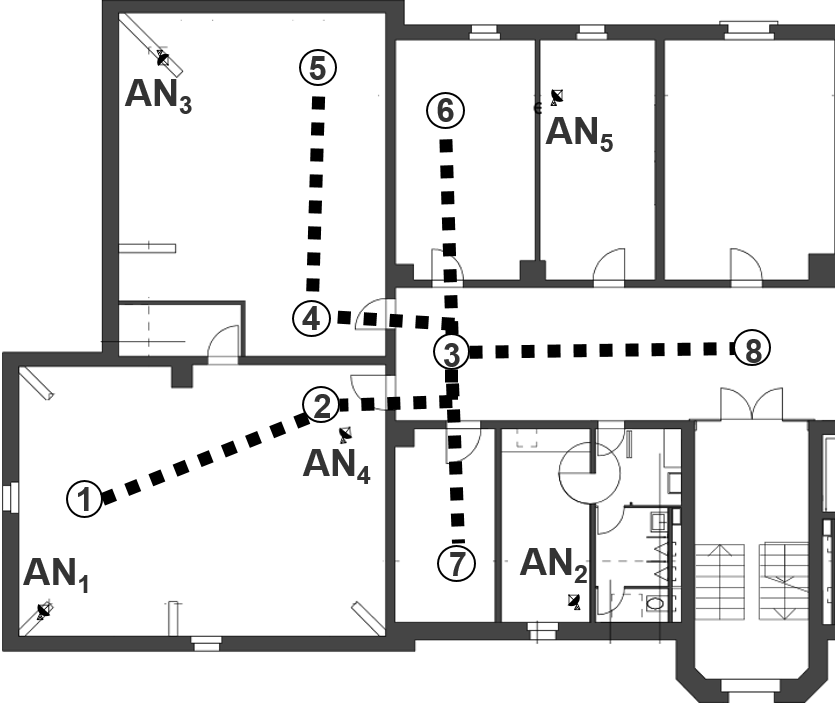
\includegraphics[width=0.5\textwidth]{Figures/trajectory5_withAnchors}
\decoRule
\caption[Trajectory 5]{Trajectory 5 with improved anchor positions.}
\label{fig:trajectory5_withAnchors}
\end{figure}
The localization error was determined by the Euclidian distance between the systems position estimation and the real position of the checkpoint.\\
\noindent\hspace*{5mm}%
For the zone detection in our algorithm, we defined 14 zones, which corresponded to 13 different rooms, where only one room (the corridor) was split into two zones. The room definitions can be seen in Figure \ref{fig:zone_definition}. For scenario 1 we collected data in all zones, whereas for the smaller scenario we only collected data in rooms 1, 2, 3, 5, 6 and 7, as only these were in the area of interest. The received signal strength values of all five UWB ANs as well as of eight Wi-Fi access points were taken into account. In order to reduce errors introduced by changing environmental conditions, we used relative RSS rather than raw RSS values. This means, we defined a pivot AN and access point and fed the machine learning algorithms with RSS difference to these given pivot RSS values and not the directly measured RSS values. In our scenarios, the AN 4 and the neighboring WiFi access point 8 were acting as a pivot (see Figure \ref{fig:trajectory1_withAnchors} and Figure \ref{fig:wifi_accessAppendix} for the exact positions). In the offline phase, we collected around 700 fingerprint measures per room. Half of them were collected randomly passing the room and half of them were collected while systematically walking through the whole area of the room.
\begin{figure}[th]
\centering
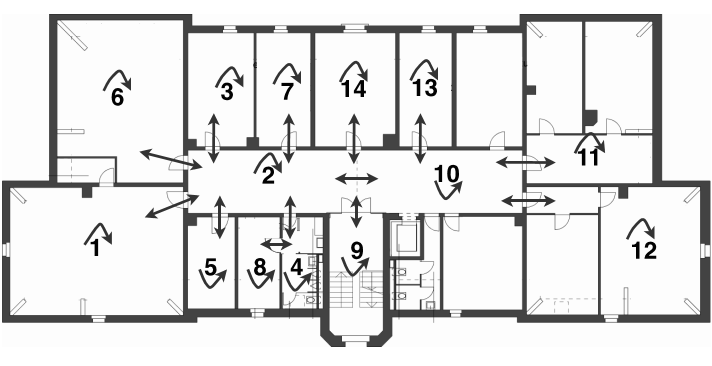
\includegraphics[width=1.0\textwidth]{Figures/zone_definition}
\decoRule
\caption[Zone Definition]{Zone definition and transitions between zones}
\label{fig:zone_definition}
\end{figure}

\section{Experiment Results}
Experiments were first conducted in scenario 1, then we covered a smaller area with a higher density of anchor nodes and conducted the experiments in scenario 2. As a reference, we compared our localization approach to a commercial localization system proposed by UNISET, called Sequitur InGPS Lite. In the following, we compare our particle filter results to the Sequitur system results.
\subsection{Localization Performance in Scenario 1}
In the following, the results of our algorithms with a wide distance between anchor nodes are shown. We called this setup scenario 1. Scenario 1 consisted of the wide anchor node positioning indicated in Figure \ref{fig:trajectory1_withAnchors}. In scenario 1 we tested four different trajectories, the trajectories 1-4. Trajectory 1 is indicated in Figure \ref{fig:trajectory1_withAnchors}, the trajectories 2, 3 and 4 are shown in Figure \ref{fig:trajectories2to4}.
\begin{figure}[th]
\centering
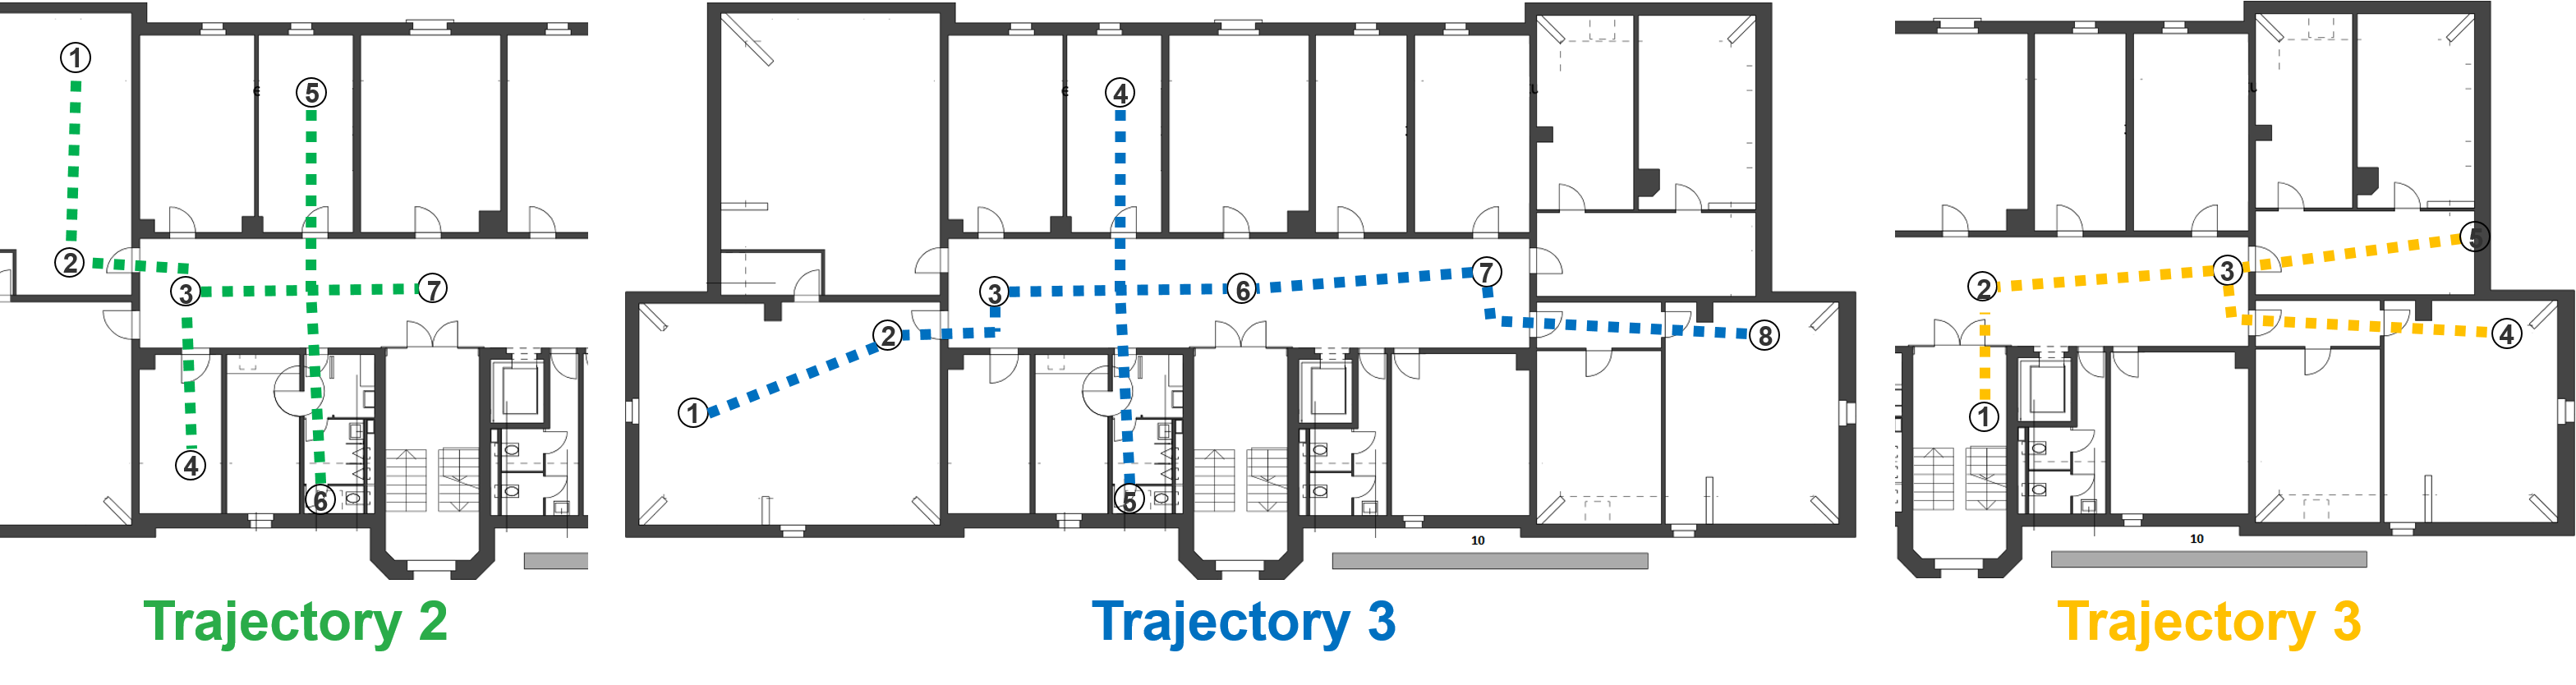
\includegraphics[width=1.0\textwidth]{Figures/trajectories2to4}
\decoRule
\caption[Trajectories 2-4]{Checkpoint position in Trajectories 2, 3 and 4}
\label{fig:trajectories2to4}
\end{figure}
The results are shown as arithmetic means of the five probes we registered.\\
\noindent\hspace*{5mm}%
In the first trajectory, the arithmetic mean (hereafter often called average) distance error over all checkpoints was $1.62$m for the particle filter and $1.75$m for Sequitur's commercial system. Looking at Figure \ref{fig:trajectory1and2_results}, we see that the errors are often smaller than $1.5m$, however, there are some checkpoints (e.g. checkpoint 5 in trajectory 1) with very low accuracy. This is also emphasized by comparing the arithmetic mean error to the median error of $1.12m$ for PF and $1.13m$ for Sequitur. The median errors are significantly lower than the arithmetic mean errors. The measurements for trajectory two looked rather similar but with a higher error. The arithmetic mean error for the PF was $2.39m$ and for Sequitur $2.35m$. The median errors were again a lot more accurate with $1.59m$ for PF and $1.16m$ for Sequitur.
\begin{figure}[th]
\centering
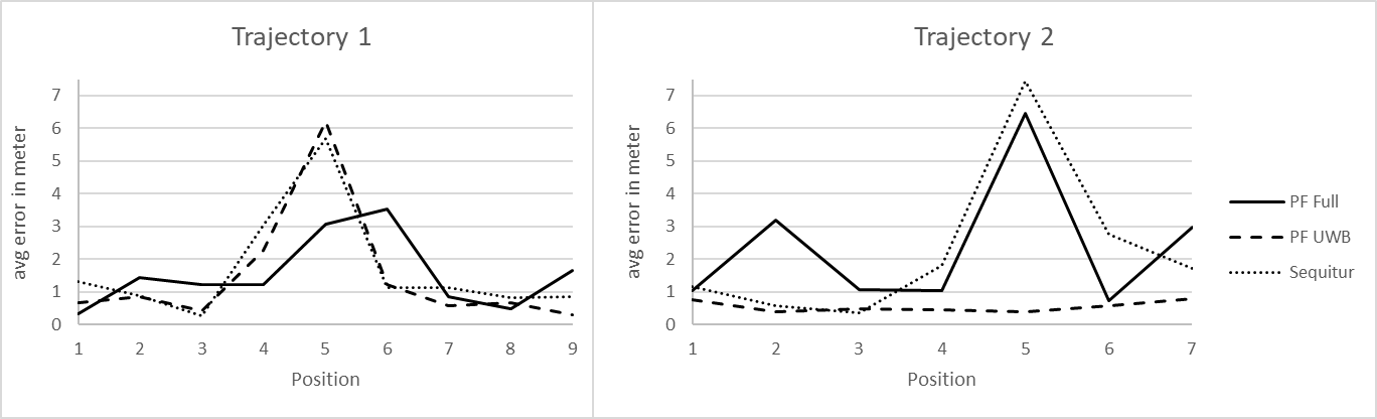
\includegraphics[width=1.0\textwidth]{Figures/trajectory1_2_results}
\decoRule
\caption[Localization Results of Trajectory 1 and 2]{Measured distance errors at each checkpoint in trajectory 1 and 2.}
\label{fig:trajectory1and2_results}
\end{figure}
The results for trajectory 3 and 4 were rather similar, however, the peaks observed in Figure \ref{fig:trajectory3and4_results} were not as extreme as for the first two trajectories. As above, the average errors in the third trajectory of $1.23m$ (PF) and $1.94m$ (Sequitur) were also considerably higher than the medians of $0.95m$ and $0.80m$.
\begin{figure}[th]
\centering
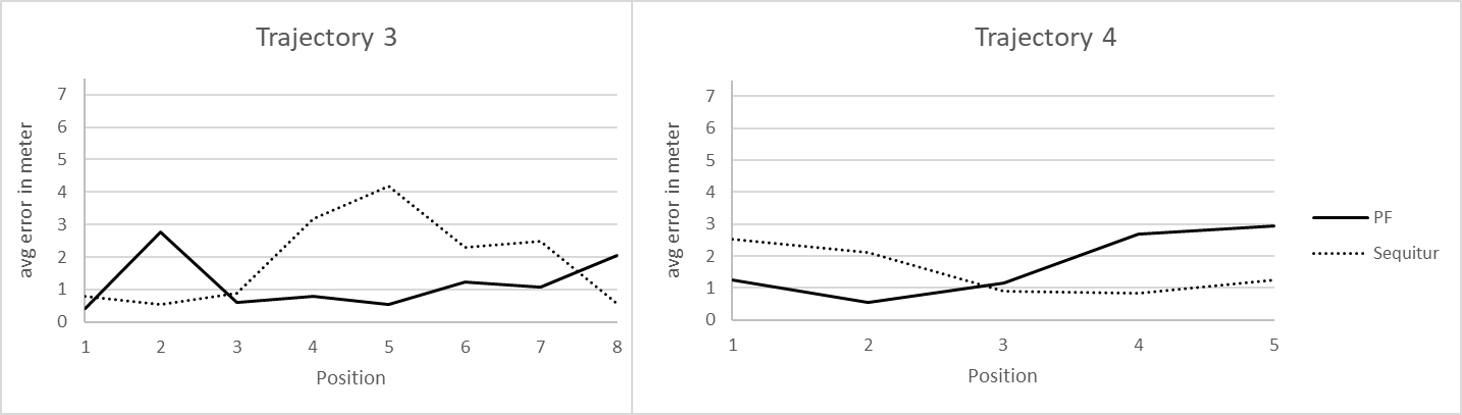
\includegraphics[width=1.0\textwidth]{Figures/trajectory3_4_results}
\decoRule
\caption[Localization Results of Trajectory 3 and 4]{Measured distance errors at each checkpoint in trajectory 3 and 4.}
\label{fig:trajectory3and4_results}
\end{figure}In the last of these four trajectories, no big outliers were stated. Nonetheless, the average errors of $1.79m$ and $1.55m$, as well as the median errors $1.24m$ and $1.26m$ for the PF and Sequitur, were still not as accurate as intended.\\
\noindent\hspace*{5mm}%
Having a closer look at Table \ref{tab:arithmetic_errors}, we see that there are very big differences between different trajectories. The particle filter and the Sequitur system have similar accuracies, for some trajectories, one of the algorithms is better, for other trajectories the other performs better. Possible reasons for these volatile results are discussed in the upcoming subsection  \ref{Section2} about result analysis. 

\begin{table}
\caption{Arithmetic Mean of Errors in Trajectories 1 to 4 (meter).}
\label{tab:arithmetic_errors}
\centering
\begin{tabular}{l l l}
\toprule
\textbf{Trajectory} & \textbf{PF} & \textbf{Sequitur}\\
\midrule
\textbf{T1} & 1.72 & 1.75\\
\textbf{T2} & 2.39 & 2.35\\
\textbf{T3} & 1.23 & 1.94\\
\textbf{T4} & 1.79 & 1.55\\
\midrule
\textbf{Total 1-4}  & \textbf{1.73} & \textbf{1.93}\\
\bottomrule\\
\end{tabular}
\end{table}

%----------------------------------------------------------------------------------------
%	SECTION 2
%----------------------------------------------------------------------------------------

\subsection{Localization Performance in Scenario 2}
For scenario 2 the density of anchor nodes was increased. We used 5 ANs for an area of 358$m^2$, which corresponds to an area of 72$m^2$ per anchor node (compared to 143$m^2$ per AN in scenario 1). In scenario 2 we tested trajectory 5, which covered already the whole area. The exact setup in scenario 2 and the checkpoints of trajectory 5 was indicated above in Figure \ref{fig:trajectory5_withAnchors}. Equally as before the results are shown as arithmetic means of the five test repetitions.\\
\noindent\hspace*{5mm}%
The results in this setup were by far better than in the setup with a lower density of ANs. With an average error of $0.49m$ for the PF and $0.48m$ for Sequitur, this setup outperformed the other trajectories with both algorithms. Even the median errors - with $0.44m$ and $0.48m$ -  were not much different, which means that there are no huge differences over the different checkpoints. This can also be seen in Figure \ref{fig:trajectory5_results}, where most of the errors are smaller than $0.80m$.

\begin{figure}[th]
\centering
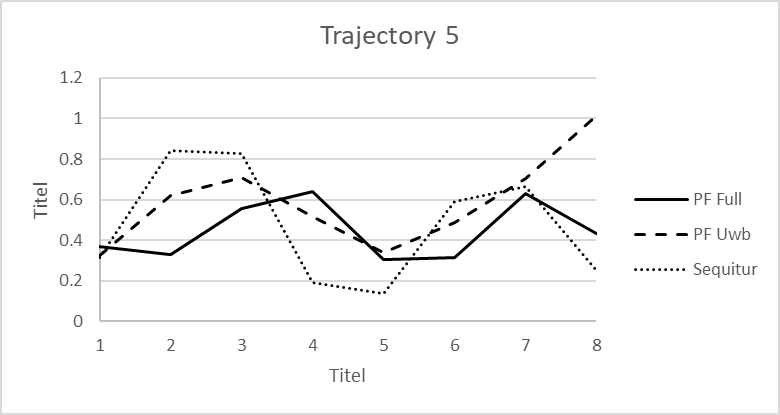
\includegraphics[width=0.8\textwidth]{Figures/trajectory5_results}
\decoRule
\caption[Positioning Results Trajectory 5]{Graph of measured distance errors at each checkpoint in trajectory 5.}
\label{fig:trajectory5_results}
\end{figure}

\begin{table}
\caption{The Arithmetic Mean of Errors in Trajectory 5 (meter).}
\label{tab:arithmetic_errors_trajectory5}
\centering
\begin{tabular}{l l l}
\toprule
\textbf{Trajectory} & \textbf{PF} & \textbf{Sequitur}\\
\midrule
\textbf{Total 1-4} & 1.73 & 1.93\\
\textbf{T5} & 0.49 & 0.48\\
\midrule
\textbf{Difference}  & \textbf{-1.24} & \textbf{-1.45}\\
\bottomrule\\
\end{tabular}
\end{table}
In Table \ref{tab:arithmetic_errors_trajectory5}, the mean errors of the low density AN scenario 1 and the high density AN scenario 2 are compared. The results improved significantly with a denser anchor node positioning. 
\begin{table}
\caption{Comparison of Scenario 1 and 2}
\label{tab:results_trajectory5}
\centering
\begin{tabular}{l l l l}
\toprule
\textbf{Algorithm} & \textbf{Mean error}[m] & \textbf{SD}[m] & \textbf{90\% Acc.}\\
\midrule
\textbf{PF (Scen 1)} & 1.729 & 1.451 & 3.393\\
\textbf{Sequitur (Scen 1)} & 1.928 & 2.337 & 5.544\\
\midrule
\textbf{PF (Scen 2)} & 0.491 & 0.239 & 0.875\\
\textbf{Sequitur (Scen 2)} & 0.484 & 0.271 & 0.829\\
\bottomrule\\
\end{tabular}
\end{table}
The standard deviation (SD) for scenario 2 was rather small with $0.24m$ for the PF and $0.27m$ for the Sequitur system, whereas the 90\% accuracy was $0.87m$ and $0.82m$. 
\begin{figure}[th]
\centering
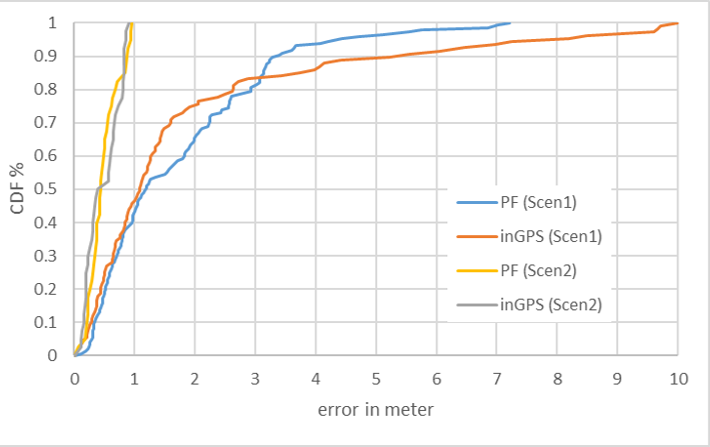
\includegraphics[width=0.8\textwidth]{Figures/cdf_all}
\decoRule
\caption[CDF Scenario 1 and 2]{The cummulative distribution function of the errors.}
\label{fig:cdf_all}
\end{figure}

\begin{figure}[th]
\centering
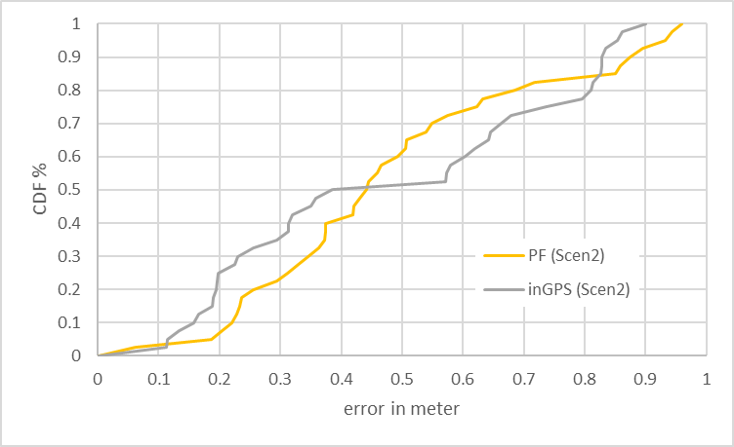
\includegraphics[width=0.8\textwidth]{Figures/cdf_scenario2}
\decoRule
\caption[CDF Scenario 2]{Zoomed cummulative distribution for scenario 2.}
\label{fig:cdf_scenario2}
\end{figure}
%----------------------------------------------------------------------------------------
%	SECTION 3
%----------------------------------------------------------------------------------------

\subsection{Result Analysis}
\label{Section2}
The test results in the experiment setup with wide anchor node distances were not very accurate. To find the reasons for that, we have to carefully have a look at the underlying implementation and the single checkpoint circumstances. We identified two main causes for bad results. These were:
\begin{itemize}
\item Some checkpoints were lying outside of AN bounding boxes.
\item UWB connection failed many times due to too wide distances from the TAG to the ANs
\end{itemize}
A cluttered environment will heavily distort UWB communication and thus affect the RTT used for UWB ranging. As in our testing environment servers with iron racks, desks with computer screens as well as a lot of different equipment was present. This effect should not be neglected.\\
\noindent\hspace*{5mm}%
The AN positions naturally form a bounding box around the environment. The bounding box is the area spanned by straight connections between anchor nodes, as indicated in Figure \ref{fig:trajectory1_boundingBox}. Trilateration, also with small distance errors, works well within the bounding box. However, even small ranging errors can lead to wrong position estimations outside the bounding box. 
\begin{figure}[th]
\centering
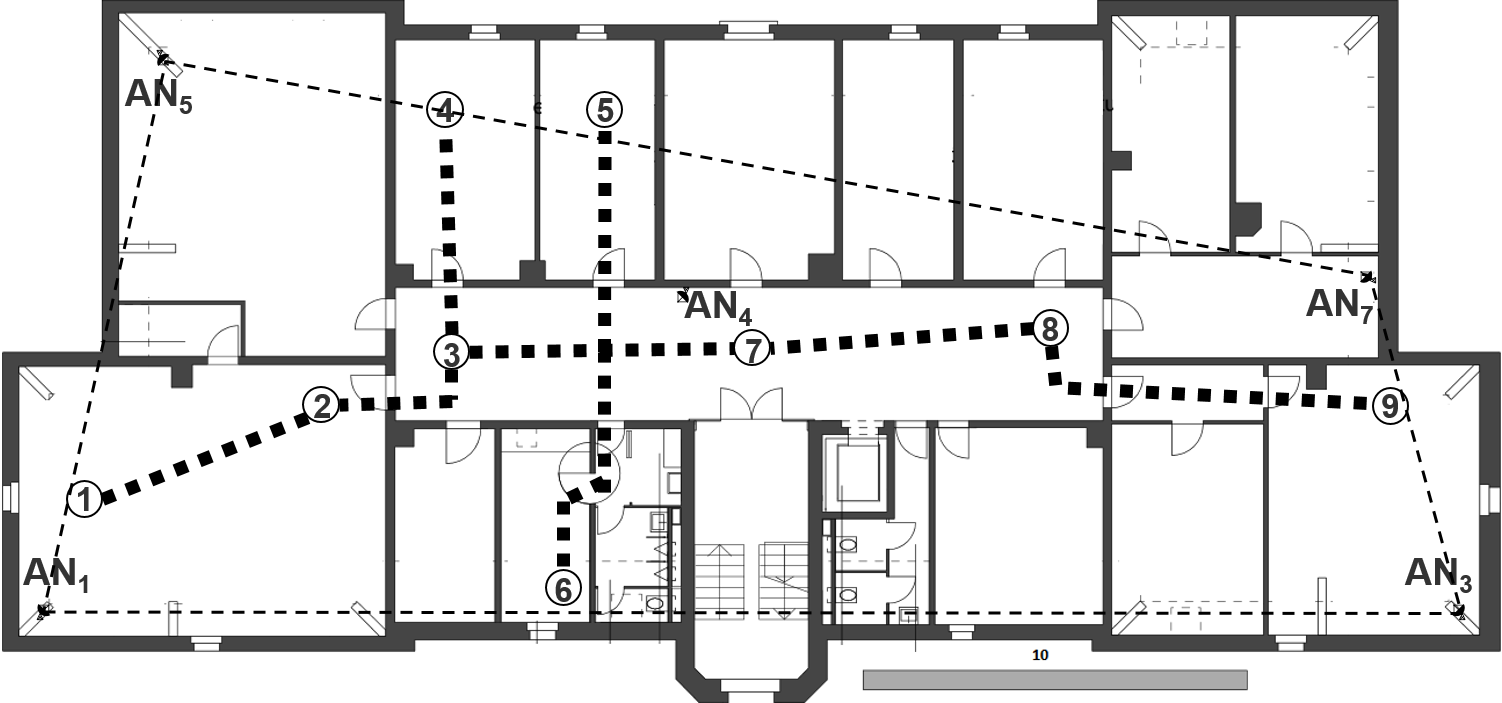
\includegraphics[width=0.8\textwidth]{Figures/trajectory1_boundingBox}
\decoRule
\caption[Bounding Box and Checkpoints for Trajectory 1 ]{Indicated bounding box of the anchor node positions for trajectory 1.}
\label{fig:trajectory1_boundingBox}
\end{figure}
In our experiment, especially the results on checkpoint 5 in trajectory 1 and 2 stand out. The average measured errors of $3.09m$ for PF and $5.70m$ for Sequitur for the first trajectory as well as $6.46m$ and $7.45m$ for the second trajectory are way higher than for other checkpoints. The fact that both algorithms had troubles estimating the position of checkpoint 5 in trajectory 1, leads to the conclusion that the experimental setup was the main reason for the big errors at this checkpoint. Moreover, besides lying outside the bounding box, this position was also far away from the nearest ANs without a direct line of sight.\\
\noindent\hspace*{5mm}%
Both algorithms depend on a well-established UWB connection, as all the ANs ranging estimations were transmitted using UWB messages. Especially in the particle filter, many UWB messages are transmitted, because fingerprinting and IMU data are additionally requested and exchanged. For certain checkpoints, the distance to the farthest anchor node was even more than $35m$ in scenario 1, which was too much for a stable UWB connection within our environment. Particularly, the particle filter had troubles receiving enough usable data, as it produced more overhead than the Sequitur system, because the particle filter transmitted IMU sensor data in addition to UWB ranging information. This led to a high packet loss, such that only one or two range measurements per estimation step were taken into account - instead of the possible five - leading to a higher error. \\
\noindent\hspace*{5mm}%
These surprisingly big inaccuracies of both systems prompted the change in our setup, in order to establish better communication between the nodes with less packet loss to enforce more data flowing into the particle filter. This was the main reason why we extended our experiments and evaluated the location accuracy in scenario 2.\\
\noindent\hspace*{5mm}%
With the more dense spread of the ANs, the estimations improved a lot. Having a look at our two assumptions above, we can state the following:

\begin{itemize}
\item Checkpoints outside of AN bounding boxes had quite a good accuracy, what contradicts our assumption.
\item The communication was better, what improved the accuracy a lot and confirmed our assumption.
\end{itemize}

In the new setup, we intentionally added checkpoints at the edge or outside of the bounding box, as seen in Figure \ref{fig:trajectory5_boundingBox}. Especially checkpoint 5 and 8 are not lying within the bounding box, however, they still had a quite good accuracy. For checkpoint 5, the average estimation errors were $0.30m$ and $0.14m$, for checkpoint 8 the errors were $0.43m$ and $0.25m$ for PF, respectively Sequitur.
\begin{figure}[th]
\centering
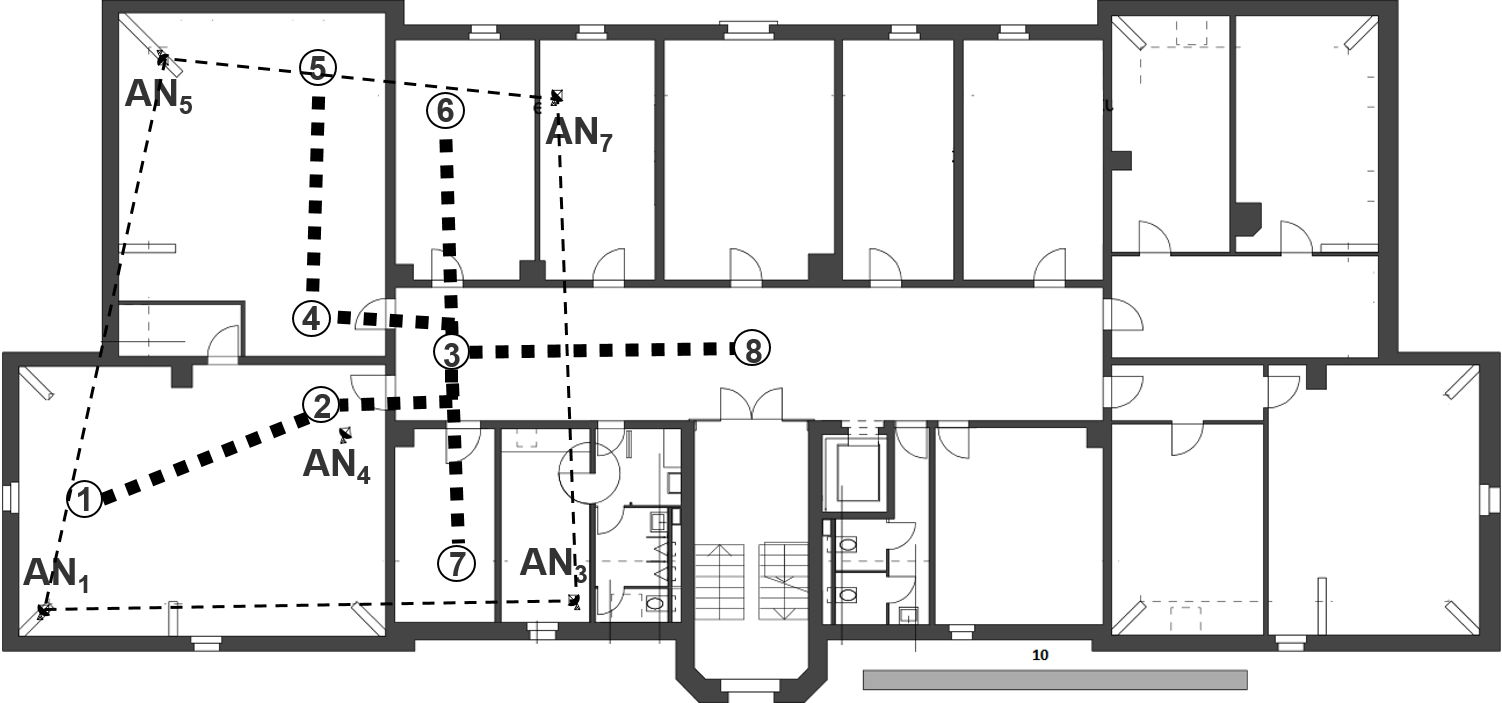
\includegraphics[width=0.8\textwidth]{Figures/trajectory5_boundingBox}
\decoRule
\caption[Trajectory 5 with Bounding Box]{Indicated bounding box of the anchor node positions for trajectory 5.}
\label{fig:trajectory5_boundingBox}
\end{figure}
It did not make a difference for the TAG being outside the bounding box or not. We conclude that it is not very important to stay within the bounding box, especially when good ranging data is available. However, when the measured ranges to the ANs contain big errors, the system is able to compensate those errors better when the TAG is within the bounding box. \\
\noindent\hspace*{5mm}%
The UWB connection had a bigger influence on the estimation error than the bounding box. With a better-established connection - in our case with nearer ANs - we had a lower packet loss. The result was, that in each estimation step, more data was available for the positioning algorithms. This led to a better accuracy.\\
For the particle filter, the communication to the ANs is very important, because the data is requested serially. Serial communication only allows a limited number of retransmissions and the communication timeouts have to be kept short. Packet loss affects the data quality, such that some evaluating steps had to be performed with fewer measurement values. Obviously, the lack of measurement values led to bad results, as the particle filter improves its estimation by fusing many different measurements, which is not possible when a part of the data is not present.